\documentclass[a4paper, 11pt, oneside]{article}
%-- Packages for shaping --%
\usepackage[utf8x]{inputenc}
\usepackage[french]{babel} 
\usepackage{lmodern}
\usepackage[T1]{fontenc}
\usepackage{fullpage}
\usepackage{graphicx}
%---------------------------------%

%----Document Informations-----%
\makeatletter
\def\clap#1{\hbox to 0pt{\hss #1\hss}}%
\def\ligne#1{%
\hbox to \hsize{%
\vbox{\centering #1}}}%
\def\haut#1#2#3{%
\hbox to \hsize{%
\rlap{\vtop{\raggedright #1}}%
\hss
\clap{\vtop{\centering #2}}%
\hss
\llap{\vtop{\raggedleft #3}}}}%
\def\bas#1#2#3{%
\hbox to \hsize{%
\rlap{\vbox{\raggedright #1}}%
\hss
\clap{\vbox{\centering #2}}%
\hss
\llap{\vbox{\raggedleft #3}}}}%
\def\maketitle{%
\thispagestyle{empty}\vbox to \vsize{%
\haut{}{\@blurb}{}
\vfill
\vspace{1cm}
\begin{flushleft}
\usefont{OT1}{ptm}{m}{n}
\huge \@title
\end{flushleft}
\par
\hrule height 4pt
\par
\begin{flushright}
\usefont{OT1}{phv}{m}{n}
\Large \@author
\par
\end{flushright}
\vspace{1cm}
\vfill
\vfill
\bas{}{\@location, le \@date}{}
}%
\cleardoublepage
}
\def\date#1{\def\@date{#1}}
\def\author#1{\def\@author{#1}}
\def\title#1{\def\@title{#1}}
\def\location#1{\def\@location{#1}}
\def\blurb#1{\def\@blurb{#1}}
\date{19 Septembre 2015} 
\blurb{}
\makeatother
\title{Phishing-WLAN}
\author{Authors}
\location{Vannes}
\blurb{%
Ecole Nationale Supérieure de Bretagne Sud\\
Spécialité Ingénieur en Cyberdéfense
}%
%---------------------------------%

\parindent=0cm

\begin{document}

\maketitle

%\tableofcontents

\section*{Introduction}
Our goal is to get the victim's credentials while he is trying to connect to a website.
This project takes place in our network course. 
The aim of this project is to practice and learn how a particular aspect of a network works.

This project can be sum up by several steps :
\begin{itemize}
\item[-] Scan the Network and choose a victim\\
\item[-] Setup a MITM Attack on the Local Area Network\\
	\begin{itemize}
    \item[-] ARP Spoofing\\
    \item[-] DNS Spoofing\\
    \item[-] steal SSL certificate\\
    \end{itemize}
\item[-] Steal credentials\\
\end{itemize}

\section{What we are doing}

\subsection{Global Process}
The first step of this attack is to look for a target by scanning the network, and getting his network gateway. \\
\begin{figure}[!h]
	\centering
	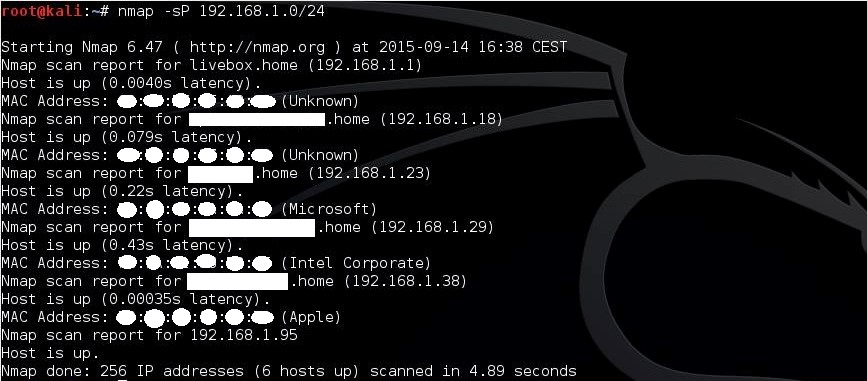
\includegraphics[scale=0.75]{../images/captureNMAP.jpg}
	\caption{nmap capture} %la légende
	\label{nmap_capture} %l'étiquette
\end{figure}
Then, we can make the target's routing table think that we are its gateway via ARPSpoofing, and redirect all the DNS requests with some DNSSpoofing.\\
For the target, this is just a normal browsing over the internet.\\
For the attacker, he can see all the packets and get any information about the target.\\


\subsubsection{ARP Step}
Before spoofing the target, we can lookup on his ARP table and see the relation between IP adress and MAC adress. \\
With those informations, we can get the AP IP and MAC adress. \\
\begin{figure}[!h]
	\centering
	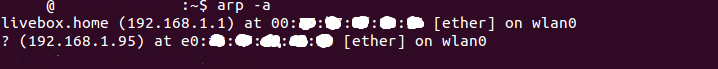
\includegraphics[scale=0.75]{../images/arpTableBeforeSpoof.png}
	\caption{ARP Table before spoof}
	\label{ARP_before_spoof}
\end{figure}

\begin{figure}[!h]
	\centering
	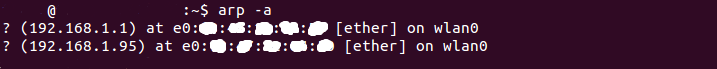
\includegraphics[scale=0.75]{../images/arpTableAfterSpoof.png}
	\caption{ARP Table after spoof}
	\label{ARP_after_spoof}
\end{figure}
We can now start the ARPSoofing, this will have the effect of sending continuously the same ARP packets (level 2 messages) to the target.\\
The point in doing this, is to force the target to think that the gateway we are sending in the ARP messages is his gateway.\\
If we open wireshark to sniff the network, we are able to see a lot of those ARP messages from the attacker.\\

Example of an ARP spoof message: 
\begin{center}
\begin{verbatim}
<MAC_PIRATE> tell <MAC_TARGET> that <IP_GATEWAY> is at <MAC_PIRATE>
\end{verbatim}
\end{center}

\begin{figure}[!h]
	\centering
	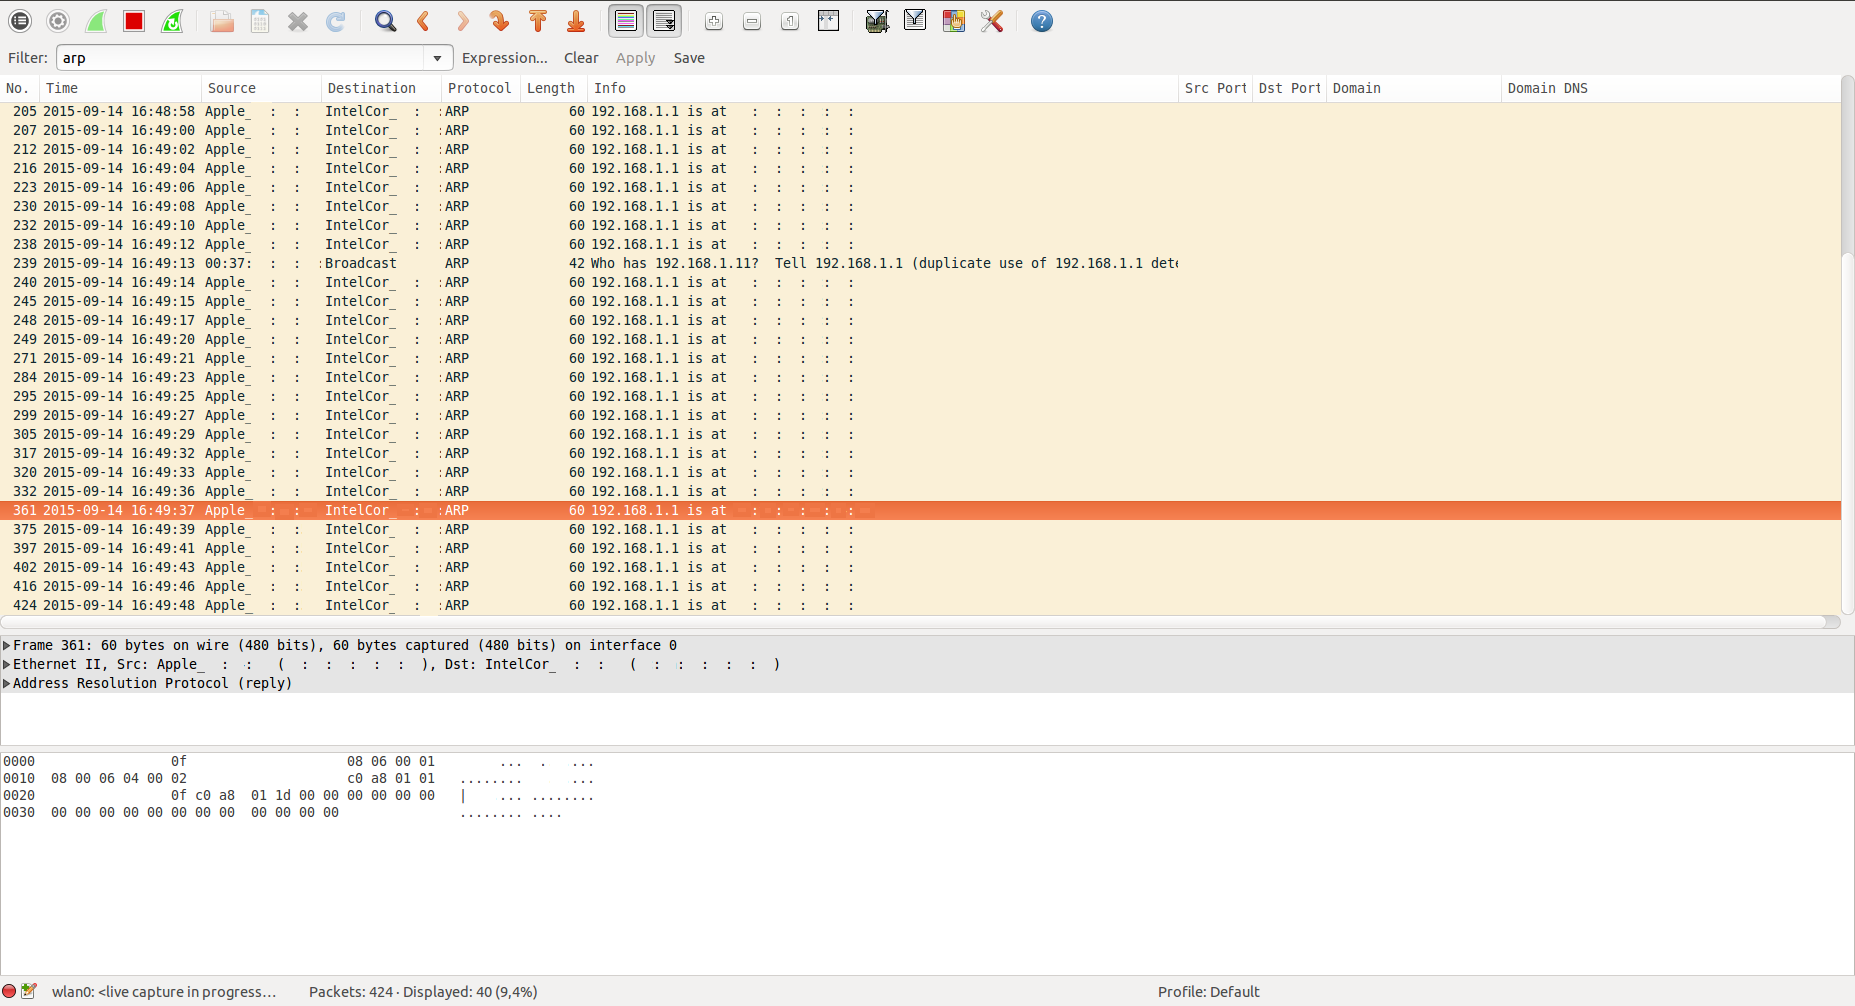
\includegraphics[scale=0.3]{../images/wiresharArpSpoof.png}
	\caption{Wireshark capture of the ARP spoofing}
	\label{Wireshark_ARP_Spoof}
\end{figure}

Then, if we look to the target's ARP table, we can see that he uses our gateway.\\
At this point, the target can't reach the internet since he is asking to our gateway.\\
To make him communicate throw the attacker's gateway, we need to activate the IP forwarding.\\
So now, the target can surf on the internet, the MITM is in place, the hacker can see what is comming throw his connections.\\

\subsubsection{DNS Step}
This step is necessary to exploit a MITM attack.\\
The purpose of the DNSSpoofing is to intercept the target's DNS requests to be able, if required, to redirect them.\\
\begin{figure}[!h]
	\centering
	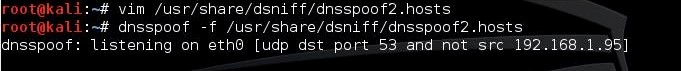
\includegraphics[scale=0.80]{../images/dnsSpoof.jpg}
	\caption{DNS spoofing}
	\label{DNS_spoofing}
\end{figure}

\subsection{What we did to legally test security flaw}
\begin{itemize}
    \item[-] Work on a personnal WLAN\\
    \item[-] Every test was ran on our personnal machines\\
\end{itemize}

\subsection{Counter measures to prevent this kind of attack}
For the website owner : \\
\begin{itemize}
    \item[-] not providing an HTTP version of his website\\
    \item[-] acquire a legitimate HTTPS certificate\\
\end{itemize}

For the internet user : \\
\begin{itemize}
    \item[-] always browse on a secured network you trust (ie not on a public WI-FI)\\
    \item[-] always browse on a HTTPS website with trusted and verified certificate\\
\end{itemize}

\section{Encountered problems}

\subsection{What they were}
\begin{itemize}
    \item[-] HTTPS protocol, while in the MITM, we can 'read' everything as long as the target is on HTTP. If we ask for HTTPS website, all the packets are protected. \\
    \item[-] HTTPS with SSLStrip, Even with ssltrip, we still have problems to get credentials on specific websites (facebook.com and gmail.com for exemple). Those website, do not use http at all, so sslstrip does not have eny effects.\\
\end{itemize}

\subsection{How we actually dealt with them}
\begin{itemize}
    \item[-] HTTPS protocol, the solution to get readable informations with this protocol is to use SSLStrip.\\
    \item[-] HTTPS with SSLStrip, we can't use it on facebook.com or gmail.com, we have to find an other website with less protection.\\
\end{itemize}
    
\section{Differences with the Overview's Objectives}

\subsection{What are those differences (if any)?}
\begin{itemize}
    \item[-] We wanted to get the credentials from gmail, but since this site is well protected against this sort of attack, we can't use it as our target.\\
\end{itemize}

\subsection{Why did we not met our objectives.}

\subsection{What are the possible solutions to meet them.}
\begin{itemize}
    \item[-] Find a website less protected and/or having http and https protocols.\\
\end{itemize}

\section{What we wanted to learn with this project and what did we really learn}
We wanted to learn how to use some basic tools provided natively with kali linux.\\

\section{How did we share the code}
We used Git (and especially GitHub) to share the code. (https://github.com/as3nds/fishing-WLAN)\\
We also used c9.io to work in a collaborative way.\\

\pagebreak

\section*{Definitions :}
\paragraph{AP}
Acces Point, device necessary to connect client on a wireless network.\\

\paragraph{MITM}
Man In The Middle, this attack is based on relaying secretly the communication between a client and the AP.\\

\paragraph{ARP Table}
It's a database with all the relation between IP adress and MAC adress.\\

\section*{Used Programs :}
\paragraph{nmap}
Scan the network in order to find a target\\

\paragraph{arpspoof}
Allows to usurp the target's gateway\\

\paragraph{wireshark}
Network analyzer, shows all the packets flowing on the network including protocols and many informations\\

\paragraph{dnsspoof}
Listen and intercept the target's DNS requests in order to apply a fake DNS table.\\

\paragraph{sslstrip}
This tool, used in a MITM attack, can change requests protocols from HTTPS to HTTP. Only works with website that have HTTP 'AND' HTTPS connection\\

\end{document}